As shown in homework F.5, the feedback linearized model for the longitudinal dynamics is given by 
\begin{equation}\label{eq:soln_g6_1}
( m_c + 2 m_r)\ddot{\tilde{h}} = \tilde{F}
\end{equation}
Taking the Laplace transform of Equation~\eqref{eq:soln_g6_1} and setting all initial conditions to zero we get
\[
( m_c + 2 m_r)s^2H(s) = \tilde{F}(s).
\]
Solving for $H(s)$ and putting the transfer function in monic form gives
\begin{equation}\label{eq:soln_g6_2}
H(s) = \frac{\left(\frac{1}{m_c + 2 m_r}\right)}{s^2}\tilde{F}(s).
\end{equation}
where the expression in the parenthesis is the transfer function from $\tilde{F}$ to $\tilde{h}$, where $\tilde{F}$ indicate that we are working with feedback linearized control derived in homework F.5. The block diagram associated with Equation~\eqref{eq:soln_g6_2} is shown in Figure~\ref{fig:hw_vtol_longitudinal_block_diagram}
\begin{figure}[htbp]
   \centering
   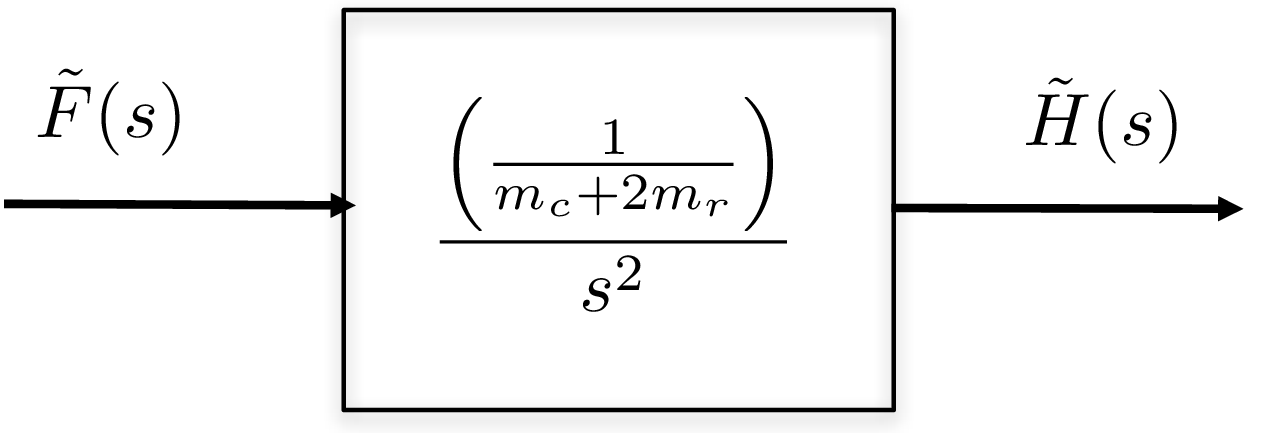
\includegraphics[width=0.5\textwidth]{6_design_studies/figures/hw_vtol_longitudinal_block_diagram.pdf}
   \caption{A block diagram of the longitudinal dynamics of the planar VTOL system.}
   \label{fig:hw_vtol_longitudinal_block_diagram}
\end{figure} 


From HW~F.5, the linearized equations of motion for the lateral dynamics are given by
\begin{align*}
(m_c+2m_r)\ddot{z} &= -F_e\tilde{\theta} - \mu\dot{\tilde{z}} \\
(J_c + 2 m_r d^2)\ddot{\tilde{\theta}} &= \tilde{\tau}
\end{align*}
Taking the Laplace transform gives
\begin{align}
\left( m_c + 2 m_r \right) s^2 \tilde{Z}(s) &= -F_0 \tilde{\Theta}(s) - \mu s \tilde{Z}(s) \label{eq:soln_g6_3}\\
\left( J_c + 2 m_r d^2 \right) s^2 \tilde{\Theta}(s) = \tilde{\tau}(s). \label{eq:soln_g6_4}
\end{align}
In matrix form we have
\[
\begin{pmatrix}
\left( m_c + 2 m_r \right) s^2 +\mu s & F_e \\
0 &  \left( J_c + 2 m_r d^2 \right) s^2
\end{pmatrix} \begin{pmatrix} \tilde{Z}(s) \\ \tilde{\Theta}(s) \end{pmatrix} 
= \begin{pmatrix}
0 \\ 1
\end{pmatrix} \tilde{\tau}(s).
\]
Defining
\begin{align*}
a_1 &\defeq m_c + 2 m_r \\
a_2 &\defeq J_c + 2 m_r d^2
\end{align*}
and inverting the matrix on the left gives
\begin{align*}
\begin{pmatrix}\tilde{Z} \\ \tilde{\Theta} \end{pmatrix}
&= \begin{pmatrix}
	a_1 s^2 + \mu s & F_0 \\ 0 & a_2 s^2 \end{pmatrix}^{-1} \begin{pmatrix} 0 \\ 1 \end{pmatrix}\tilde{\tau}(s) \\
&= \frac{\begin{pmatrix}
	a_2 s^2 & -F_0 \\ 0 & a_1 s^2 + \mu s\end{pmatrix}}{a_2s^2(a_1s^2+\mu s)} \begin{pmatrix} 0 \\ 1 \end{pmatrix} \tilde{\tau}(s) \\
&= \frac{\begin{pmatrix} -F_0 \\ a_1 s^2 + \mu s \end{pmatrix}}{a_2s^2(a_1s^2+\mu s)}\tilde{\tau}(s) \\
&= \begin{pmatrix} \frac{-\left(\frac{F_0}{a_1a_2}\right)}{s^3(s+\frac{\mu}{a_1})} \\ \frac{\left(\frac{1}{a_2}\right)}{s^2}\end{pmatrix}\tilde{\tau}(s),
\end{align*}
which are the transfer function from $\tau$ to $\tilde{z}$ and $\tilde{\theta}$.  

Returning to Equations~\eqref{eq:soln_g6_3} and~\eqref{eq:soln_g6_4} note that the system is naturally in cascade form.
From Equation~\eqref{eq:soln_g6_4} the transfer function from $\tilde{\tau}$ to $\tilde{\theta}$ is 
\[
\tilde{\Theta}(s) = \frac{\left(\frac{1}{a_2}\right)}{s^2}\tilde{\tau}(s).
\]
Similarly, from Equation~\eqref{eq:soln_g6_3}, the transfer function from $\tilde{\theta}$ to $\tilde{z}$ is
\[
Z(s) = \frac{-\left(\frac{F_0}{a_1}\right)}{s\left( s+ \frac{\mu}{a_1}\right)} \tilde{\Theta}(s).
\]

Therefore, the block diagram for linearized lateral subsystem is shown in Figure~\ref{fig:hw_vtol_lateral_block_diagram}
\begin{figure}[htbp]
   \centering
   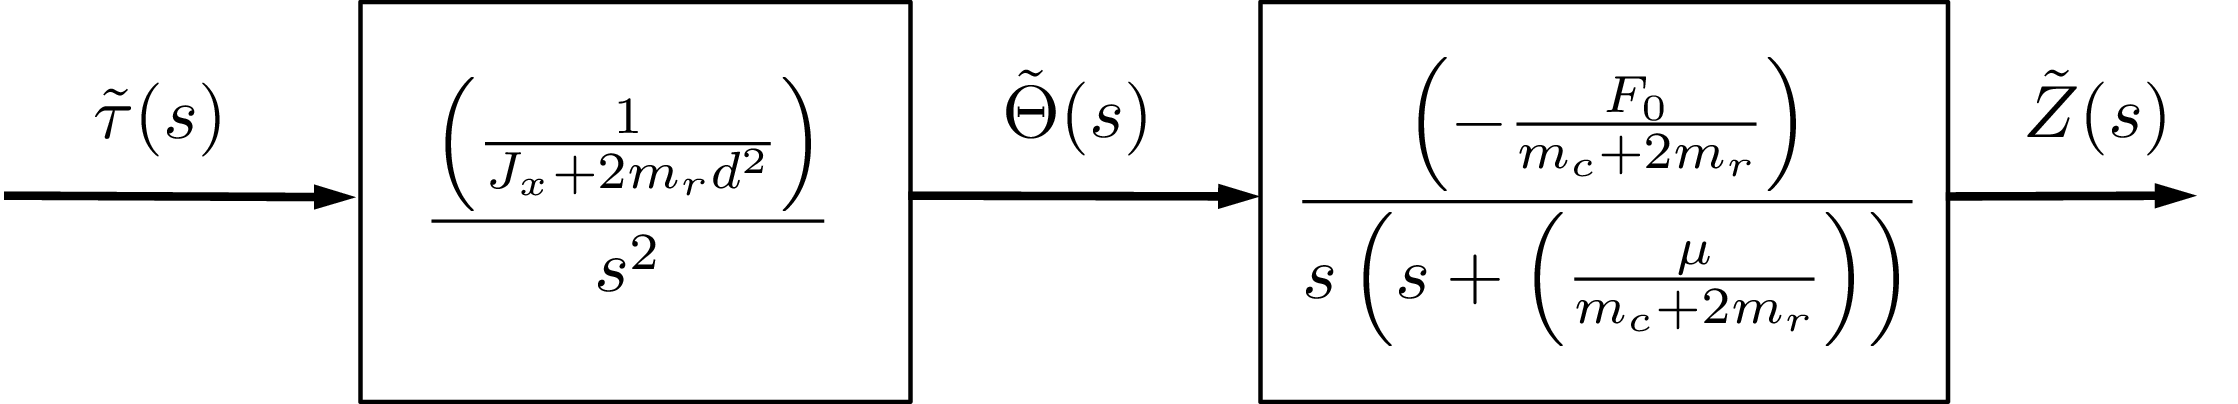
\includegraphics[width=0.8\textwidth]{6_design_studies/figures/hw_vtol_lateral_block_diagram.pdf}
   \caption{A block diagram of the lateral dynamics of the planar VTOL system.}
   \label{fig:hw_vtol_lateral_block_diagram}
\end{figure}

The cascade approximation makes since physically because the torque on the planar VTOL system has an almost immediate effect on the angle of the aircraft, which leads to side to side motion.
